\chapter{Machine Learning System Design and Evaluation}
\label{ml}

This chapter presents the design and architecture of the machine learning system used in \nplh.  This system is comprised of three components: an information retrieval system, a classifier for {\tt Pet} artifacts, and a classifier for {\tt Match} artifacts.  The information retrieval system is implemented in {\em pylucene}\footnote{http://lucene.apache.org/pylucene/}, which is a Python wrapper around the popular Lucene search engine.  The {\tt Pet} and {\tt Match} classifiers are designed to observe volunteer activity (in the form of utilizing the artifacts they produce) and render judgments on the respective artifacts they handle; the output of these classifiers is used to modify the rankings produced by querying the information retrieval system.

The public interface of this system, detailed in the previous chapter, is relatively simple and intended to allow consumers of this system to be very agnostic about its implementation.  While this is, in general, a good software engineering principle to follow, the generic public interface is also important because the architecture of this system is still in many ways a prototype.  The information retrieval system and classification framework are simple in design and intended to provide a baseline for both system design and the evaluation of the features used in these components.  The concluding chapter of this work discusses future directions for development of this system.

The following sections discuss the design of the three primary system components and how they are combined to produce ranked query responses for the {\tt matching} application.  The remainder of the chapter is dedicated to detailing evaluations of the components individually and as a whole in an experimental setting.

\section {Design Considerations}

The classifiers included in this system are designed to incorporate ongoing training as the activities of digital volunteers are observed.  This is essential to the agential positioning of the machine computation performed by the system; it is key that the system adapts to new information coming from (human) collaborators over time.  Because of this, the machine learning algorithms used in the system are supervised rather than unsupervised, meaning that they are trained using labeled data that act as training examples \cite{jurafsky:nlp}.  This is not to say that unsupervised algorithms are unsuitable for this domain, but simply that the supervised approach better synthesizes with the human activity taking place within the system.

Furthermore, because the system must adapt over time, the algorithms used must be capable of retraining and thereby adjusting their internal probabilistic models in response to new data (a process known as {\em active learning}).  Essentially this means the classifier must either keep all of its training examples stored or be able to adjust its model using stored statistics (in the case of a probabilistic classifier).  The latter method is preferred for performance reasons and can be accomplished in a variety of ways depending on the classification algorithm \cite{jurafsky:nlp, sebastiani:ml}.  In practice, \nplh{} would likely perform active learning in batch processes (again, for performance reasons) rather than use a pure online approach to retraining.

Finally, because the classifiers are ultimately used to modify ranked retrieval results from an information retrieval system, and thus are ultimately not being used to make ``hard'' decisions \cite{sebastiani:ml}, these classifiers have different requirements than traditional textual classification systems.  Several environmental conditions play a significant role in the design and evaluation of these classifiers:

\begin{itemize}
  \item{} The quality of the training data is not guaranteed to be high for many reasons: 
  \begin{itemize}
  		\item{} Data generation in the system is relatively unrestricted and the correctness of a pet report, in terms of grammar, spelling, and adherence to format (i.e., putting only breed information in a ``breed'' field) cannot be assured.  
  		\item{} Although digital volunteers can improve poor pet reports by editing them, they are not directed, trained annotators and thus training examples cannot be expected to have consistent characteristics across their entire population.  
  		\item{} The nature of the problem domain makes textual classification inherently difficult (see Chapter 2).  
  \end{itemize}
  \item{} The central problem in matching pets is that there is {\em at most} one correct pet in the system.  This generally means that the classifiers in the system must favor {\em recall} (or {\em sensitivity} in this context) over {\em precision}; it is paramount that the classifier correctly categorize the true positive, if it exists.  False positives can be forgiven easily as long as the true positive improves in terms of its search ranking.  Again, we can rely on human computation (and subsequent verification by the crowd) to solve the hard problem as long as the machine learning components are helping to reduce the problem of large search spaces.
\end{itemize}

\section {Lucene Index}

The core component of the machine learning systems is, somewhat misleadingly, actually an information retrieval system.  The {\tt matching} application must present a ranked list of suggested pets to a user in response to a selected pet; this process is directly analogous to querying a search engine for a list of relevant documents (with the caveat that in this system there is at most one relevant document to any query).  Using this analogy, {\tt Pet} artifacts can easily be viewed as multi-field documents to be indexed in an information retrieval system.

As mentioned in this chapter's introduction, \nplh{} implements this information retrieval system as a Lucene index.  {\tt Pet} artifacts are translated to multi-field documents (i.e., the {\tt breed} property on a {\tt Pet} artifact is translated into a corresponding field in the Lucene document).  Lucene processes these documents (using Lucene's {\tt SimpleAnalyzer} tokenization method) and stores relevant information about the documents and their terms, like {\em tf} $\cdot$ {\em idf} scores.  

When the {\tt matching} application presents a {\tt Pet} artifact to this subsystem, the supplied pet report is translated into a Lucene query using multi-field query syntax.  The only hard matching requirement set on this query is for the {\tt lost} field, which indicates whether or not the report is for a lost or found pet (this value is set to the opposite of the supplied artifact's value).  The query is executed using Lucene's standard searching tools ({\tt IndexSearcher}) and a ranked list of documents (pet reports) is returned.  This ranked list is then reordered according to the scoring formula (describe later in this chapter) to obtain a final ranking which is then returned to the {\tt matching} application.

\section {{\tt Pet} Classifier Architecture}

The objective of the {\tt Pet} classifier is to obtain some measure of the quality and completeness of a given pet report.  This information is assumed to be valuable because a pet report that is incomplete or of poor quality is less likely to be matched in general than one that is of high quality and fully described.  

This component is designed as a simple binary classifier which labels a {\tt Pet} artifact as either positive or negative.  A positive label indicates that the pet report is of high quality and completeness, and a negative label indicates the opposite.  In practice, the scoring function utilizes the probability that the {\tt Pet} artifact belongs to the positive class:

\[
	p(C_1 | F) = \frac{p(C_1)p(F | C_1)}{p(F)}
\]
where $F$ is a feature vector representing the pet report, and $C_1$ is the positive class.

This classifier is Bayesian, as can be seen in the formula above.  The feature vector representation of a pet report is implemented as a bag of words, with each term in the vocabulary represented by a particular index in the one-dimensional vector; this is a standard model used in information retrieval and text classification \cite{jurafsky:nlp, manning:ir}.  

One feature of the {\tt Pet} artifact does not directly translate to a binary feature --- this is the {\tt revisions} attribute, which tracks user judgments and edits to a pet report, and is intuitively the most important feature for this classifier.  We can translate this feature into numeric form by counting the number of revisions with no edits (which act as upvotes to the pet report).  This number can be made even more interesting when multiplied by the social capital of the users involved (and properly normalized), making its potential value as a distinguishing feature even greater.

Still, this number is not compatible with a bag-of-words feature vector.  The simplest way to resolve this problem is to assign a distinct token in the vocabulary for each occurring value of this number, but this approach is problematic.  A better approach is to stratify the possible values of this number into distinct tokens in the vocabulary \cite{macskassy:text}.  For example, a numeric value ranging between 0 and 100 might be discretized into four separate tokens, ``{\tt zero, over10, over30, over70}''.  This approach has the advantage in that the tokens created can be more meaningfully selected and result in information gain.

I have thus far neglected to mention the specific classification algorithm that this classifier implements.  This is because, in the interest of exploration, I have evaluated various algorithms for this classifier.  These variations include two Naive Bayes classifiers (multinomial and Bernoulli), a Support Vector Machine (SVM), a Nearest Neighbors classifier, and a Decision Tree classifier.  The classifier described above fits the description of a Naive Bayes classifier because these classifiers best fit the design requirements described in this chapter; they can be designed for active learning, and in addition, they exhibit high bias, which performs well with the relatively small amounts of data present in the system.  I will discuss the evaluation of these various algorithms later in the chapter.

\section {{\tt Match} Classifier Architecture}

Like the {\tt Pet} classifier, the {\tt Match} classifier is implemented as a Bayesian classifier (though, like the {\tt Pet} classifier, I evaluate several different classification algorithms for this component).  The goal of this classifier is to examine a pair of pet reports and render a judgment about whether or not the pair constitutes a likely match or not.  This information is naturally assumed to be valuable to the process of ranking potential matches for the {\tt matching} application.  In many ways this classifier acts as a collaborative filter, using successful matches to try to discover other potential matches.

Unlike the {\tt Pet} classifier, the {\tt Match} classifier does not directly include textual tokens into its feature vector.  Instead, the feature vector examines the similarity of the two pet reports on a field by field basis.  The specific information in each pet report which is considered is breed, color, size, sex, age, and description.  Before comparison, the strings contained in each field are cleaned, removing punctuation and character case.  After this, the fields are then tokenized and placed into a set to facilitate comparison.  Each field comparison results in two features - whether or not the corresponding fields are disjoint, and the number of overlapping tokens in each field, normalized by field length, which results in the percentage of overlapping tokens.  This latter feature is then stratified like the {\tt revisions} attribute was for the {\tt Pet} classifier, using the same methodology \cite{macskassy:text}.  This stratification results in six separate features.  Combined with the feature which categorizes disjointness, this entire process creates a feature vector with 42 binary features.

It is notable that this classifier does not actually consider the content of the pet reports, as does the {\tt Pet} classifier.  This is by design; the training data for matches is extremely limited, rendering content classification less useful.  Furthermore, the content of pet reports is, intuitively, not actually that useful to determining whether or not they constitute a good match.  For example, two similar reports about a labrador retriever are not a good potential match because they are about labrador retrievers; they are a good potential match because they are both about the same breed of animal.  By considering only the similarity of the fields between the two pet reports, this classifier seeks to discover what the most useful correlations are within individual pet reports.

\section {Combined Scoring System}

Using the three components of this system, I define a combined scoring system that produces the rank of a given pet report in relation to another pet report.  In practice, the system uses this scoring system to reorder the ranked results of a Lucene query, as discussed previously.  The most complete scoring algorithm (in the sense that it utilizes all the components of the system) is as follows:

\begin {equation}
S(P_1, P_2) = L(P_1, P_2) \times \frac{C_P(P_1) + C_P(P_2)}{2} \times C_M(P_1, P_2)
\label{eq:scoring}
\end {equation}
where $P_1$ is the query pet report, $P_2$ is a potential matching pet report, $L(P_1, P_2)$ is the original Lucene score for the pair, $C_P(x)$ is the {\tt Pet} classifier's probability estimate that $x$ belongs to the positive class, and $C_M(P_1, P_2)$ is the {\tt Match} classifier's probability estimate that the pair is a match.

It should be noted that the probability estimates given by each classifier are true probability estimates because of the need for normalization (probability estimates produced by classifiers are usually just scores because there is often no need for this normalization if the classifier is used independently). 

Formula~\ref{eq:scoring} utilizes all possible components of the system.  However, because the evaluation of this system is exploratory, I have evaluated several variations of this scoring formula for the combined evaluation of the system discussed at the end of this chapter.  These variations are described by Table~\ref{table:scoring}.

\begin{table}[htb]
    \caption[Variations of the scoring formula]{
	This table details the variations of the general scoring formula which are used in the combined evaluation of this system.
	}
		\small
    \begin{center}
    % four columns - .25, .1, .15, .6
    \begin{tabularx}{ \textwidth}{| c | p{10cm} | X | } 
    \hline
    	Name & Equation & Description \\  \hline \hline
			
			$S_1$ & 
			\[ S_1(P_1, P_2) = L(P_1, P_2) \times \frac{C_P(P_1) + C_P(P_2)}{2} \times C_M(P_1, P_2) \] &
			Identical to the general formula; incorporates all components of the system.	\\ \hline
			
			$S_2$ & 
			\[ S_2(P_1, P_2) = L(P_1, P_2) \times \frac{C_P(P_1) + C_P(P_2)}{2} \] &
			Does not utilize the {\tt Match} classifier.	\\ \hline
			
			$S_3$ & 
			\[ S_3(P_1, P_2) = L(P_1, P_2) \times C_P(P_2) \] &
			Does not utilize the {\tt Match} classifier or the {\tt Pet} classifier's score for $P_1$.	\\ \hline
			
			$S_4$ & 
			\[ S_4(P_1, P_2) = L(P_1, P_2) \times C_M(P_1, P_2) \] &
			Does not utilize the {\tt Pet} classifier.	\\ \hline
	\end{tabularx}
   \\ \rule{0mm}{5mm}
	\end{center}
	 \label{table:scoring}
\end{table}


\section {Experimentation and Evaluation}

The evaluation of this system is two-fold, incorporating both individual evaluations of each classifier as well as a combined evaluation which examines how well the scoring formulas (described in the previous section) improve the rankings of true positive matches in ranked results.  The following sections describe the structure of these evaluations, discussing the corpus and methods used to obtain labeled training data, as well as the specific implementation details of various classification algorithms.

Evaluation of both the individual classifiers and the combined system was always performed through 10-fold cross validation.  Experimental results for the individual classifiers are presented in terms of these folds, as well as aggregated metrics.  Although fold results are presented in terms of accuracy figures, the more important metrics are the overall precision, recall, and $F_2$ score for the classifiers.  Because of the emphasis on recall, I chose to calculate the $F_2$ measure, which is a variation of the harmonic mean of precision and recall which weights recall higher than precision.

\subsection {Corpus}

The problem domain of pet-to-family reunification is very different from traditional textual classification domains; finding an appropriate corpus of data was difficult.  Many online services which index reports of lost pets do not also index reports of found pets, which have semantic differences.  Ultimately I used publicly available data obtained from ``America's National Lost \& Found Pet Database''\footnote{http://www.lostfoundpets.us/} (operated by the Alabama Pet Registry) as a raw corpus of lost and found pets.

\begin{figure}[htbp]
    \begin{center}
	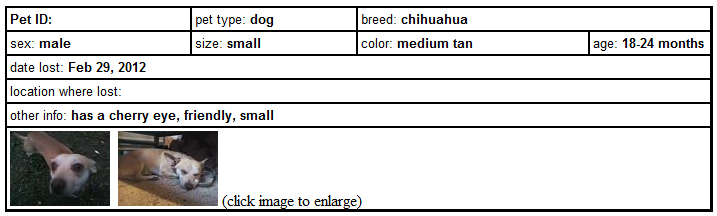
\includegraphics[width=125mm]{figs/corpus.png}
    \end{center}
        \caption[Sample Pet in Corpus]{
        Sample pet obtained from corpus.
	}
	 \label{fig:corpus}
\end{figure}

Figure~\ref{fig:corpus} displays a (censored) sample entry from this database.  Entries in this database contain information about pet type, breed, sex, size, color, age, date lost or found, location lost or found, a field for ``other information'', and one or more pictures of the pet.  Although interesting (and possibly useful for future work), I removed information regarding location and date as the pets retrieved from the database were spread geographically across the United States and wide range of dates, which is not realistic for a disaster event.  Furthermore, the ``other information'' field varied widely in terms of its content, ranging from being empty to containing multiple paragraphs of grammatically incorrect, irrelevant information.

I immediately removed from my corpus those pets which did not have pictures attached to their reports.  This cut down the size of the corpus from just over 2000 reports to just over 800 reports.  The distribution between lost and found pet reports was approximately even, so I was able to leave this initial corpus fairly in tact barring the changes discussed above.

\subsection {Classifier Implementation}

Classifiers were implemented in Python using the {\em scikit-learn} machine learning library \cite{scikit-learn}.  This library supports many classification algorithms and offers support for evaluation and experimentation.  Table~\ref{table:algorithms} details the various classification algorithms used in evaluating the {\tt Pet} and {\tt Match} classifiers.

\begin{table}[htb]
    \caption[Classifier implementations]{
	This table details the various classification algorithms that were used as implementations for the {\tt Pet} and {\tt Match} classifiers.
	}
    \begin{center}
    % four columns - .25, .1, .15, .6
    \begin{tabularx}{ \textwidth}{| l | l | X | } 
    \hline
    	ID & Algorithm & Notes \\  \hline \hline
			MNB & Multinomial Naive Bayes & Variant of Naive Bayes that permits non-binary features (preserves term counts for the {\tt Pet} classifier). \\ \hline
			BNB & Bernoulli Naive Bayes & Assumes features are binary-valued; binarizes feature vectors (discards term counts for the {\tt Pet} classifier). \\ \hline
			KNN & K-Nearest Neighbors & $k$ defaults to 5. \\ \hline
			DT & Decision Tree & Utilizes Gini impurity as the splitting algorithm. \\ \hline
	\end{tabularx}
   \\ \rule{0mm}{5mm}
	\end{center}
	 \label{table:algorithms}
\end{table}

\subsection {{\tt Pet} Classifier Training}

To obtain labeled training examples of complete, high-quality and incomplete, low-quality pet reports, I constructed an annotation application to allow volunteers to evaluate and edit pet reports in the corpus.  Ten volunteers, selected from a convenience sample, assisted in this annotation process.  This application's interface is shown in Figure~\ref{fig:annotation1}.

\begin{figure}[htbp]
    \begin{center}
	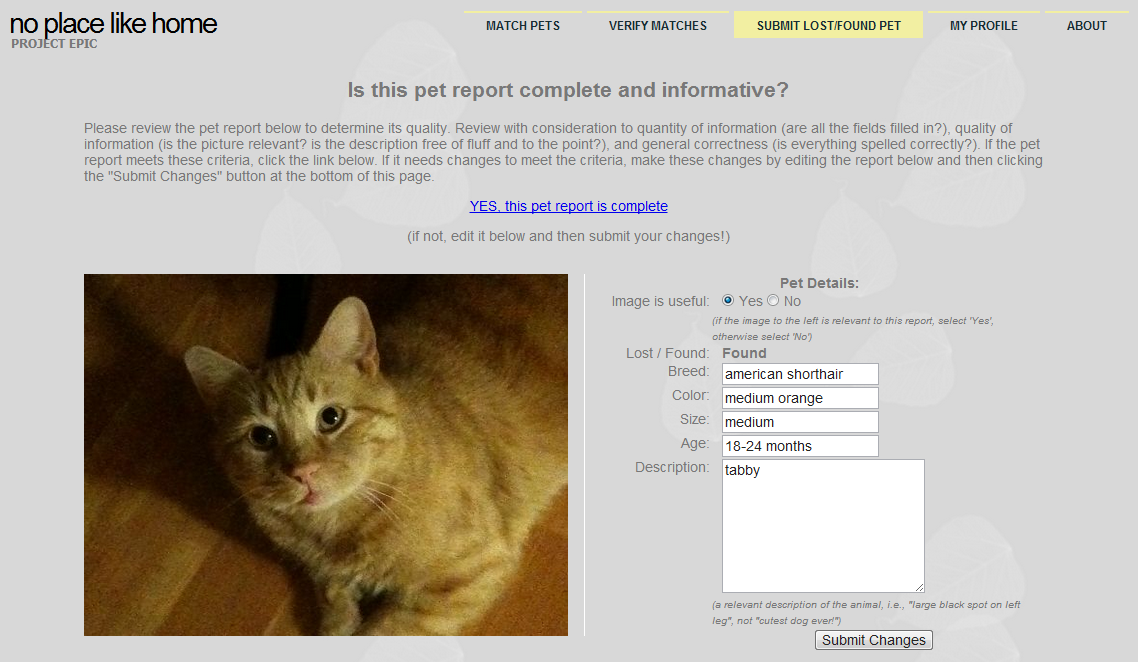
\includegraphics[width=150mm]{figs/annotation1.png}
    \end{center}
        \caption[{\tt Pet} classifier Annotation Interface]{
        Interface allowing volunteers to edit or upvote pet reports (this interface is utilizing the {\tt reporting} application).  
	}
	 \label{fig:annotation1}
\end{figure}

The annotation application asks volunteers to render their judgment on whether or not the pet report is complete and informative and provides brief annotation instructions, such as checking the spelling of the content of the pet report.  If the volunteer feels the pet report is of high quality, they can register an upvote for that report.  If the report is lacking, the volunteer can edit the pet report and submit a new revision of it.  After submitting an upvote or a revision, the annotation application would display a new pet report at random to the user.

The majority of pet reports in the original corpus received revisions rather than upvotes; these revisions usually took the form of either spelling corrections or major changes to the description field.  Annotators were instructed that this field should contain a concise, relevant description of the animal that encompassed features not captured by the other fields.  For example, a good description might be ``Dog has white chest and large black spot on back left leg; long hair.''

Because this field was initially populated with the ``other information'' field obtained from the raw corpus, however, it often contained information that was irrelevant to the pet, such as contact information, or sentimental text.  Although both of these have a place in \nplh{}, these fields obscure the classification process and annotators removed this irrelevant information.

Pet reports that were upvoted became positive training examples.  If a revision was made to a pet report by an annotator, the previous version of the pet report was used as a negative training example (unless that report had upvotes, which was a rare case), with the revised version being used as a positive training example.

This process resulted in over 1000 positive training examples and over 800 negative training examples being generated for use in classification.

\subsection {{\tt Pet} Classifier Evaluation}

The labeled data generated by annotators was used in 10-fold cross validation to train and evaluate the various implementations (see Table~\ref{table:algorithms}) of the {\tt Pet} classifier.  Table~\ref{table:peteval} displays the results of this evaluation.

The Bernoulli Naive Bayes classifier outperforms the other classifiers in terms of accuracy, precision, and $F_2$ score, losing the accuracy title in only two folds to the Nearest Neighbors and Decision Tree.  Overall, however, it is unsurprising that the Naive Bayes classifiers outperformed the Nearest Neighbors and Decision Tree classifiers.  As discussed before, Naive Bayes classifiers are well suited to the type and quantity of training data present in this evaluation.  

\begin{table}[htb]
    \caption[{\tt Pet} classifier evaluation]{
	This table displays the evaluation results for each implementation of the {\tt Pet} classifier.  The displayed statistic for each fold is the accuracy of that classifier for that fold.  Overall accuracy, precision, recall, and $F_2$ scores are also provided.  {\em Bolded} cells indicate the best-performing classifier for that metric.
	}
		\small
		\tabcolsep 4.5pt
    \begin{center}
    \begin{tabular}{@{}|l|*{10}{c|}|*{4}{c|}@{}}
    \hline
    & \multicolumn{10}{c||}{Folds} & \multicolumn{4}{|c|}{Mean Evaluation Metrics} \\
		\hline
		{\em ID} & 1 & 2 & 3 & 4 & 5 & 6 & 7 & 8 & 9 & 10 & Acc. & Prec. & Rec. & $F_2$ \\ \hline \hline
		MNB & .639 & {\em .707} & .611 & .615 & .615 & .716 & .668 & .553 & .611 & .659 & .639 & .524 & {\em .907} & .789 \\ \hline
		BNB & {\em .678} & {\em .707} & .615 & {\em .635} & {\em .625} & {\em .736} & {\em .678} & .563 & {\em .625} & {\em .682} & {\em .654} & {\em .536} & .900 & {\em .790} \\ \hline
		KNN & .534 & .481 & {\em .635} & .582 & .558 & .529 & .615 & .529 & .615 & .530 & .561 & .400 & .242 & .262 \\ \hline
		DT & .591 & .606 & .567 & .620 & .587 & .582 & .601 & {\em .625} & .538 & .580 & .590 & .477 & .504 & .497 \\ \hline
		\end{tabular}
   \\ \rule{0mm}{5mm}
	\end{center}
	 \label{table:peteval}
\end{table}

\subsection {{\tt Match} Classifier Training}

To obtain labeled training examples of pet matches, I extended the existing annotation application to allow users to submit pet reports which would serve as matches to pet reports within the system.  Although I had originally planned to use matches that existed in the metadata of the original corpus, I found these matches to be unsuitable for training and evaluation because they consisted largely of junk data.  I therefore set out to create synthetic ground truth data in a manner that would preserve as much ecological validity as possible.

To do this I identified lost pet reports that had more than one picture associated with their report.  The annotation application used to train the {\tt Pet} classifier only uses the first picture associated with a report; the other pictures associated with pet reports had not been seen previously by annotators.

I extended the annotation application with another interface that displays an alternate picture of a pet belonging to the aforementioned set and asks the user to submit a found pet report for that pet, using only the picture (see Figure~\ref{fig:annotation2}).  This task mirrors the actual problem facing a data scout who takes pictures of pets in a shelter or finds a pet and must describe them using (potentially) only visual information.  In fact, the data scout is at an advantage because he or she can more easily determine the size, sex, and visual characteristics of the animal in question because he or she presumably does not need to rely only on a photograph of the animal.  The annotators, unfortunately, do not possess this advantage.

\begin{figure}[htbp]
    \begin{center}
	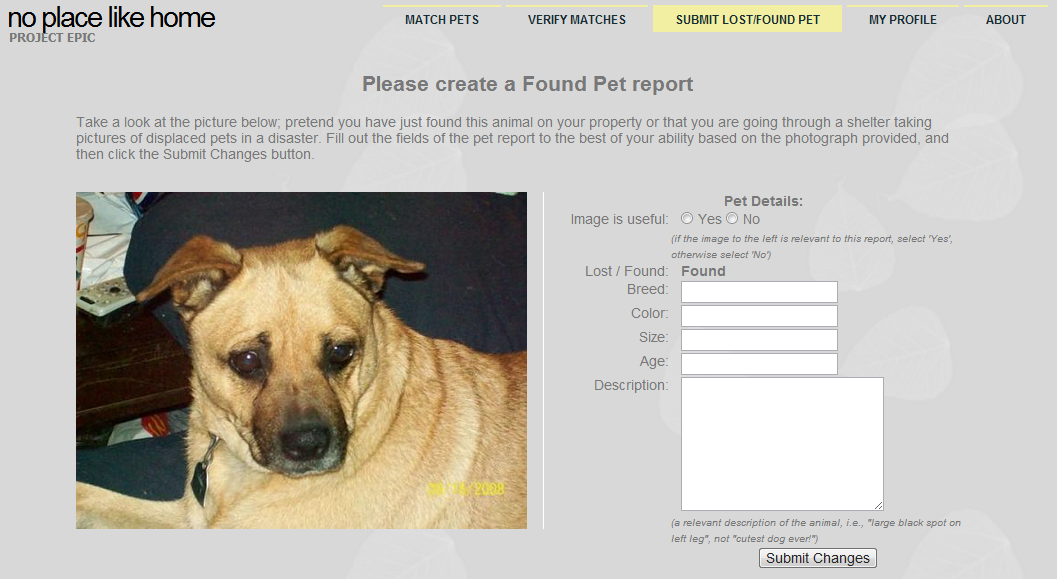
\includegraphics[width=150mm]{figs/annotation2.png}
    \end{center}
        \caption[{\tt Match} classifier Annotation Interface]{
        Interface allowing volunteers to submit a found pet report which corresponds to an existing lost pet report.  The application displays an alternate picture from the original pet report.
	}
	 \label{fig:annotation2}
\end{figure}

Annotators generated 101 ``matches'' using this interface.  The size of this set in proportion to the data set as a whole roughly corresponds to match percentages seen in real life systems (5\% to 15\% - see Chapter 2).  These matches were all used as positive training examples.  Negative training examples were created by generating a set of random matches between other pet reports outside the positive set.

\subsection {{\tt Match} Classifier Evaluation}

The labeled data generated by annotators was used in 10-fold cross validation to train and evaluate the various implementations (see Table~\ref{table:algorithms}) of the {\tt Match} classifier.  Table~\ref{table:matcheval} displays the results of this evaluation.

The accuracy metric for this evaluation is misleading in that it closely tracks the class prior probabilities (i.e., $p(C_{\text{match}}) \approx .1$).  This explains the haphazard winners of the accuracy metric across the various folds.  Again, there is good reason to believe that the most useful evaluation metric for classification in this domain is recall; here the Naive Bayes classifiers outperform the other classifiers.

Both versions of Naive Bayes perform essentially identically; this is to be expected because feature vectors provided to the {\tt Match} classifier are always binary-valued.  In practice, however, the Bernoulli Naive Bayes classifier seems best suited to this classification task.  

\begin{table}[htb]
    \caption[{\tt Match} classifier evaluation]{
	This table displays the evaluation results for each implementation of the {\tt Match} classifier.  The displayed statistic for each fold is the accuracy of that classifier for that fold.  Overall accuracy, precision, recall, and $F_2$ scores are also provided.  {\em Bolded} cells indicate the best-performing classifier for that metric.
	}
		\small
		\tabcolsep 4.5pt
    \begin{center}
    \begin{tabular}{@{}|l|*{10}{c|}|*{4}{c|}@{}}
    \hline
    & \multicolumn{10}{c||}{Folds} & \multicolumn{4}{|c|}{Mean Evaluation Metrics} \\
		\hline
		{\em ID} & 1 & 2 & 3 & 4 & 5 & 6 & 7 & 8 & 9 & 10 & Acc. & Prec. & Rec. & $F_2$ \\ \hline \hline
		MNB & .877 & .913 & .864 & {\em .930} & .852 & .877 & .901 & .951 & {\em .901} & {\em .933} & .900 & .598 & {\em .598} & {\em .592} \\ \hline
		BNB & .877 & {\em .914} & .864 & .926 & .852 & .877 & .901 & .951 & {\em .901} & {\em .933} & .900 & .598 & {\em .598} & {\em .592} \\ \hline
		KNN & .864 & .852 & .914 & .923 & {\em .914} & {\em .926} & .901 & {\em .963} & {\em .901} & .921 & .908 & {\em .710} & .412 & .444 \\ \hline
		DT & {\em .901} & .889 & {\em .938} & .901 & {\em .901} & .889 & {\em .937} & .951 & {\em .901} & {\em .933} & {\em .914} & .702 & .541 & .564 \\ \hline
		\end{tabular}
   \\ \rule{0mm}{5mm}
	\end{center}
	 \label{table:matcheval}
\end{table}

\subsection {Combined Evaluation}

In each evaluation the Bernoulli Naive Bayes implementation of each classifier outperformed the other algorithms(in terms of recall and $F_2$ score) and thus was selected as the implementation used for each classifier in the combined evaluation, which is essentially an end-to-end evaluation of the machine learning system.  This evaluation is meant to discover the effectiveness of the two classification components and how best to combine them with the results of the Lucene scorer.  This evaluation examines all the scoring algorithms in Table~\ref{table:scoring}.  

The baseline metric in this evaluation is the average and median ranking of the true positive across the set of all annotator-created matches as produced by Lucene.  The effectiveness of the various scoring functions (and consequently, that of the classification components as well) is judged by how well the average and median ranking of the true positives is improved (reduced) after re-ranking is completed.  Table~\ref{table:combined} displays the results of this final evaluation.

\begin{table}[htb]
    \caption[Combined evaluation]{
	This table displays the evaluation results for the combined, end-to-end evaluation of the various scoring functions and their components.  The rank figures shown are the mean and median ranks of the true positive across the result sets.  Percentage improvement is calculated using a result set size of 235, which was equal to the median result set size of all 101 queries (queries at most return half of the index due to the hard querying requirement splitting lost and found pet reports).  
	}
		\small
    \begin{center}
    \begin{tabular}{|l|c|c|c|c|}
		\hline
		
		{\em Scoring Function} & Mean Rank & Median Rank & \begin{tabular}[x]{@{}c@{}}\% Improvement\\to Mean Rank\end{tabular} & \begin{tabular}[x]{@{}c@{}}\% Improvement\\to Median Rank\end{tabular} \\ \hline \hline
		Lucene Baseline & 54.32 & 26 & N/A & N/A \\ \hline \hline
		$S_1$\textasteriskcentered & 54.65 & 13 & $-0.61\%$ & $50\%$ \\ \hline
		$S_2$\textasteriskcentered & 88.9 & 48 & $-63.7\%$ & $-84.6\%$ \\ \hline
		$S_3$\textasteriskcentered & 107.5 & 65 & $-97.9\%$ & $-150\%$ \\ \hline
		$S_4$\textasteriskcentered & {\em 49.39} & {\em 10} &  $9.1\%$ & $61.5\%$ \\ \hline
		\end{tabular}
   \\ \rule{0mm}{5mm}
	\end{center}
	   \textasteriskcentered Results shown are the averages across 10-fold cross validation. 
   \label{table:combined}
\end{table}

Although the baseline metric was calculated across the entire set of positive matches using just Lucene, it is important to note that 10-fold cross validation was again employed in evaluating the various scoring functions (to ensure that classifiers were never to used re-rank queries whose constituent {\tt Pet} artifacts were members of their training sets).  The recalculated rank statistics displayed in Table~\ref{table:combined} are the averages across the folds.  Furthermore, the {\tt Match} classifier uses the same set of negative training examples for this evaluation as it did in its individual evaluation to ensure consistency.

The first takeaway from these results is that generic, baseline Lucene query rankings perform fairly well to begin with; the baseline median rank of the true positive is 26.  It is important to remember that the result set size in this evaluation is fairly small (the median size being 235 results).  Furthermore, it seems useful to consider the median rank with higher regard than the mean rank, as a few outliers in the 101 queries skew the mean statistic.  Finally, I do not provide precision metrics for this ranked retrieval evaluation because it is fairly meaningless (there is at most one relevant document for any query).  However, if in the future (after ongoing interface design work is complete) an estimate for the number of pet reports that could be displayed at one time on a user's web browser became available, it would be interesting to see a precision-at-$k$ metric to evaluate whether or not the system is doing a good job at getting the true positive ``above the fold''.

It is apparent from the results of this end-to-end evaluation that the {\tt Pet} classifier was generally unhelpful in improving the rank of the true positive.  This could be due to a variety of reasons; the classifier's performance was not high enough, or the difference between the classes (complete and informative vs. incomplete and uninformative) is not pronounced enough in the labeled training data produced by volunteers.  Finally, it could be that regardless of the performance of the classifier, this information is actually not relevant to whether or not two pet reports are a good match - this would invalidate the hypothesis which is the reason for the development of this classifier.  It is interesting to note, however, that the negative impact of this classifier on the re-ranking process was greatly mitigated when combined with the results of the {\tt Match} classifier (in scoring formula $S_1$).

The {\tt Match} seems to have performed admirably in this evaluation despite displaying average performance in its individual evaluation.  The classifier appears to be able to correctly categorize the true positive in the rankings with high probability estimate (boosting the ranking of the true positive) and does a good enough job with the other results that the ranking of the true positive across the query set is improved.  Again, we see that the mean ranking is skewed by outliers, but the median rank shows significant improvement, with the $S_4$ scoring function resulting in a 61.5\% improvement in median rank of the true positive.

This result is the most promising presented in this chapter.  It is tempting to view the individual classification evaluation results and even these end-to-end evaluation results as average at best, but this is to be expected; in Chapter 2 I discussed the many challenges that this machine learning system faces.  In assessing these results, it is important to note that any improvement in the end-to-end evaluation is good, because the machine learning system is not expected to make hard decisions about what combinations of pet reports are or are not viable matches.  The system relies on the foundation of human computation to make this hard decision; its role is only to assist in this decision.